\begin{frame}[fragile]
\frametitle{Vertex Array Object (VAO)}
	\begin{itemize}
	\item Narozdíl od VBO neukládají data o vrcholech (pozice, normála, ...).
	\item VAO ukládají reference na VBO a nastavení atributů.
	\item VAO usnadňují a urychlují vykreslování.
	Pro vykreslení stačí aktivovat VAO a ten si pamatuje veškeré nastavení.
  \item V Core profile je vyžadován u každého drawcallu.
	\end{itemize}
\end{frame}

\begin{frame}[fragile]
\frametitle{VAO - použití}
	\begin{enumerate}
	\item Vygenerování jména VAO.
	\item Aktivování VAO.
	\item Vygenerování VBO, nastavení atributů.
	\item Deaktivování VAO.
	\end{enumerate}
\end{frame}

\begin{frame}[fragile]
\frametitle{VAO - použití}
  \begin{figure}[h]
  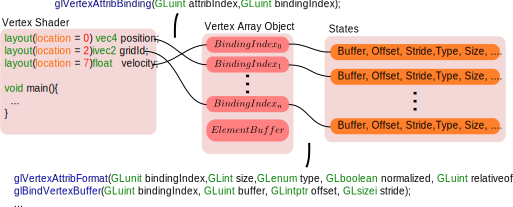
\includegraphics[width=11cm,keepaspectratio]{pics/vao.pdf}
  \end{figure}
\end{frame}

\begin{frame}[fragile]
\frametitle{VAO - příklad použití}
	Aplikace - inicializace
	{\scriptsize
	\begin{minted}[frame=lines]{c++}
	glGenVertexArrays(1,&VAO);//vygenerovani jmena VAO
	glBindVertexArray(VAO);//aktivovani VAO
	//nyni nastavime buffery a atributy
	glGenBuffers(1,&VBO);
	glBindBuffer(GL_ARRAY_BUFFER,VBO);
	glBufferData(GL_ARRAY_BUFFER,sizeof(Data),Data,GL_STATIC_DRAW);

	glGenBuffers(1,&EBO);
	glBindBuffer(GL_ELEMENT_ARRAY_BUFFER,EBO);
	glBufferData(GL_ELEMENT_ARRAY_BUFFER,sizeof(Index),Index,GL_STATIC_DRAW);

	glBindBuffer(GL_ARRAY_BUFFER,VBO);
	glEnableVertexAttribArray(vPos);
	glVertexAttribPointer(vPos,2,GL_FLOAT,GL_FALSE,sizeof(float)*5,
	  (GLvoid*)(sizeof(float)*0));

	glEnableVertexAttribArray(vCol);
	glVertexAttribPointer(vCol,3,GL_FLOAT,GL_FALSE,sizeof(float)*5,
	  (GLvoid*)(sizeof(float)*2));

	glBindVertexArray(0);//deaktivujeme VAO po tomto bode uz jej neovlivnujeme
	\end{minted}
	}
\end{frame}

\begin{frame}[fragile]
\frametitle{VAO - příklad použití}
	Aplikace - vykreslení
	{\scriptsize
	\begin{minted}[frame=lines]{c++}
	glBindVertexArray(VAO);//aktivujeme VAO
	glDrawElements(GL_TRIANGLES,6,GL_UNSIGNED_INT,NULL);
	glBindVertexArray(0);//deaktivujeme VAO
	\end{minted}
	}
\end{frame}

